\documentclass[11pt]{article}
\usepackage{amsmath, amssymb, physics, mathtools, bm}
\usepackage{tikz, pgfplots}
\pgfplotsset{compat=1.18}
\usepackage[margin=2.3cm]{geometry}
\usepackage{siunitx, booktabs, hyperref}
\usepackage{braket}

\newcommand{\D}{\mathrm{D}}
\newcommand{\de}{\mathrm{d}}
\newcommand{\pd}[2]{\frac{\partial #1}{\partial #2}}
\newcommand{\pdd}[2]{\frac{\partial^{2} #1}{\partial #2^{2}}}
\newcommand{\Lap}{\nabla^{2}}

\title{B6 Condensed-Matter Physics --- Model Solutions, Trinity 2022}
\author{}
\date{}

\begin{document}
\maketitle

%==============================================================
\section*{Question 1 --- Cu$_3$Au structure factor and powder diffraction}

\textbf{Problem.} Auricupride Cu$_3$Au, primitive cubic, $a=\SI{0.375}{nm}$, Au at corners, Cu at face centres. Derive structure factor; powder pattern at $\lambda=\SI{0.154}{nm}$; disordered alloy; partial-order parameter $\rho$.

\subsection*{(a) Structure factor and Bragg condition}

\textbf{(i) Unit cell.}
\begin{center}
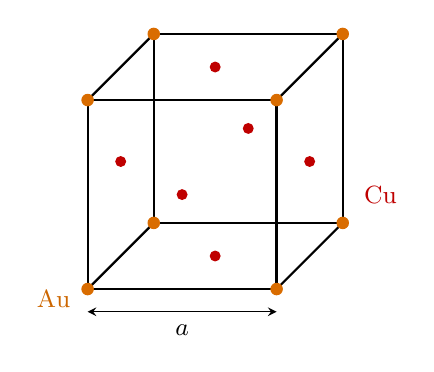
\begin{tikzpicture}[scale=2.4,>=stealth]
\coordinate (A) at (0,0);
\coordinate (B) at (1,0);
\coordinate (C) at (1,1);
\coordinate (D) at (0,1);
\coordinate (A1) at (0.35,0.35);
\coordinate (B1) at (1.35,0.35);
\coordinate (C1) at (1.35,1.35);
\coordinate (D1) at (0.35,1.35);
\draw[thick] (A)--(B)--(C)--(D)--cycle;
\draw[thick] (A1)--(B1)--(C1)--(D1)--cycle;
\draw[thick] (A)--(A1); \draw[thick] (B)--(B1);
\draw[thick] (C)--(C1); \draw[thick] (D)--(D1);
% Au corners
\foreach \p in {A,B,C,D,A1,B1,C1,D1}
  \node[circle,fill=orange!85!black,inner sep=1.6pt] at (\p) {};
% Cu face centres
\node[circle,fill=red!75!black,inner sep=1.4pt] (F1) at (0.5,0.5) {};        % front
\node[circle,fill=red!75!black,inner sep=1.4pt] (F2) at (0.85,0.85) {};      % top
\node[circle,fill=red!75!black,inner sep=1.4pt] (F3) at (1.175,0.675) {};    % right
\node[circle,fill=red!75!black,inner sep=1.4pt] (F4) at (0.175,0.675) {};    % left
\node[circle,fill=red!75!black,inner sep=1.4pt] (F5) at (0.675,0.175) {};    % bottom
\node[circle,fill=red!75!black,inner sep=1.4pt] (F6) at (0.675,1.175) {};    % back-top? actually back face
\node[orange!80!black] at (-0.18,-0.05) {\small Au};
\node[red!75!black] at (1.55,0.5) {\small Cu};
\draw[<->] (0,-0.12)--(1,-0.12) node[midway,below=1pt]{\small $a$};
\end{tikzpicture}
\end{center}

Counting per cell: $8\times\tfrac{1}{8}=1$ Au; $6\times\tfrac{1}{2}=3$ Cu. Stoichiometry Cu$_3$Au confirmed.

\textbf{(ii) Structure factor.} Basis: Au at $(0,0,0)$; Cu at $\tfrac{a}{2}(1,1,0),\tfrac{a}{2}(1,0,1),\tfrac{a}{2}(0,1,1)$. Reciprocal vector $\vb G_{hkl}=(2\pi/a)(h,k,l)$.

Definition:
\[ S_{hkl}=\sum_\alpha f_\alpha e^{i\vb G_{hkl}\cdot\vb r_\alpha}. \]
Insert basis:
\begin{equation}
S_{hkl}=f_{\text{Au}}+f_{\text{Cu}}\bigl[e^{i\pi(h+k)}+e^{i\pi(h+l)}+e^{i\pi(k+l)}\bigr].
\label{eq:Shkl}
\end{equation}
Each phase is $\pm1$:
\[ \alpha_{hkl}=e^{i\pi(h+k)}+e^{i\pi(h+l)}+e^{i\pi(k+l)}. \]
All-even or all-odd ($h,k,l$ unmixed): all three exponents even:
\[ \alpha_{hkl}=+3. \]
Mixed parity: exactly two pair-sums odd:
\begin{equation}
\boxed{\;\alpha_{hkl}=\begin{cases}+3, & h,k,l\text{ unmixed}\\ -1, & h,k,l\text{ mixed}.\end{cases}\;}
\label{eq:alpha}
\end{equation}

\textbf{(iii) Bragg's law.} Elastic: $|\vb k_f|=|\vb k_i|=2\pi/\lambda$. Laue: $\vb q=\vb k_f-\vb k_i=\vb G$. Geometry of isoceles triangle:
\[ |\vb q|=2|\vb k_i|\sin\theta_{hkl}. \]
Substitute $|\vb k_i|=2\pi/\lambda$:
\begin{equation}
\boxed{\;G_{hkl}=\frac{4\pi\sin\theta_{hkl}}{\lambda}.\;}
\label{eq:Bragg}
\end{equation}

\subsection*{(b) Powder pattern at $\lambda=\SI{0.154}{nm}$}

\textbf{(i) Scattering angles.} Cubic: $G_{hkl}=(2\pi/a)\sqrt{h^2+k^2+l^2}$. Combine with \eqref{eq:Bragg}:
\[ \sin\theta_{hkl}=\frac{\lambda}{2a}\sqrt{h^2+k^2+l^2}. \]
Numerical prefactor:
\[ \frac{\lambda}{2a}=\frac{0.154}{0.750}=0.2053. \]
$(110)$:
\[ \sin\theta_{110}=0.2053\sqrt{2}=0.2904. \]
\[ \theta_{110}=16.88^\circ. \]
\[ \boxed{2\theta_{110}\approx 33.8^\circ.} \]
$(111)$:
\[ \sin\theta_{111}=0.2053\sqrt{3}=0.3556. \]
\[ \theta_{111}=20.83^\circ. \]
\[ \boxed{2\theta_{111}\approx 41.7^\circ.} \]

\textbf{(ii) Intensity ratio.} Powder intensity (no LP, no geometry):
\[ I_{hkl}=m_{hkl}|S_{hkl}|^2. \]
Multiplicities: $m_{110}=12$, $m_{111}=8$. From \eqref{eq:Shkl},\eqref{eq:alpha}:
\begin{equation}
S_{110}=f_{\text{Au}}-f_{\text{Cu}},\qquad S_{111}=f_{\text{Au}}+3f_{\text{Cu}}.
\label{eq:S110-S111}
\end{equation}
Compute $(\sin\theta/\lambda)^2$ in $\si{nm^{-2}}$:
\[ (\sin\theta_{110}/\lambda)^2=(0.2904/0.154)^2=3.555. \]
\[ (\sin\theta_{111}/\lambda)^2=(0.3556/0.154)^2=5.331. \]
Apply $f_X=Z_X e^{-b_X(\sin\theta/\lambda)^2}$ at $(110)$:
\[ f_{\text{Cu}}^{(110)}=29\,e^{-0.063\times 3.555}=29\,e^{-0.2240}=23.18. \]
\[ f_{\text{Au}}^{(110)}=79\,e^{-0.080\times 3.555}=79\,e^{-0.2844}=59.45. \]
At $(111)$:
\[ f_{\text{Cu}}^{(111)}=29\,e^{-0.063\times 5.331}=29\,e^{-0.3358}=20.74. \]
\[ f_{\text{Au}}^{(111)}=79\,e^{-0.080\times 5.331}=79\,e^{-0.4265}=51.59. \]
Substitute into \eqref{eq:S110-S111}:
\[ S_{110}=59.45-23.18=36.27. \]
\[ S_{111}=51.59+3(20.74)=113.81. \]
Form ratio:
\[ \frac{I_{111}}{I_{110}}=\frac{8\times(113.81)^2}{12\times(36.27)^2}. \]
Evaluate squares:
\[ \frac{I_{111}}{I_{110}}=\frac{8\times 12953}{12\times 1316}. \]
Multiply:
\[ \frac{I_{111}}{I_{110}}=\frac{103620}{15788}. \]
Divide:
\[ \boxed{\;\frac{I_{111}}{I_{110}}\approx 6.6.\;} \]

\subsection*{(c) Fully disordered alloy}

\textbf{(i) Intensities.} Average form factor at every site:
\[ \bar f=\tfrac14 f_{\text{Au}}+\tfrac34 f_{\text{Cu}}. \]
Replace $f_{\text{Au}},f_{\text{Cu}}\to\bar f$ in \eqref{eq:Shkl}:
\[ S_{hkl}=\bar f\,[1+e^{i\pi(h+k)}+e^{i\pi(h+l)}+e^{i\pi(k+l)}]. \]
For $(110)$: bracket $=1+1-1-1=0$:
\[ \boxed{S_{110}=0,\quad I_{110}=0.} \]
For $(111)$: bracket $=4$:
\[ S_{111}=4\bar f=f_{\text{Au}}+3f_{\text{Cu}}, \]
identical to part (b), so $I_{111}$ unchanged.

\textbf{(ii) Extinction rules.} With one species $\bar f$ at corners and face centres, the structure is fcc with conventional parameter $a$. Fcc selection rule: $h,k,l$ unmixed allowed, mixed forbidden. Hence $(110)$ extinct; $(111)$ allowed. Reflections such as $(110)$ are \emph{superlattice} lines: present only when ordering distinguishes corner and face sublattices.

\begin{center}
\begin{tikzpicture}[scale=2.0,>=stealth]
\coordinate (A) at (0,0);\coordinate (B) at (1,0);
\coordinate (C) at (1,1);\coordinate (D) at (0,1);
\coordinate (A1) at (0.35,0.35);\coordinate (B1) at (1.35,0.35);
\coordinate (C1) at (1.35,1.35);\coordinate (D1) at (0.35,1.35);
\draw[thick] (A)--(B)--(C)--(D)--cycle;
\draw[thick] (A1)--(B1)--(C1)--(D1)--cycle;
\draw[thick] (A)--(A1);\draw[thick] (B)--(B1);
\draw[thick] (C)--(C1);\draw[thick] (D)--(D1);
\foreach \p in {A,B,C,D,A1,B1,C1,D1,(0.5,0.5),(0.85,0.85),(1.175,0.675),(0.175,0.675),(0.675,0.175),(0.675,1.175)}
  \node[circle,fill=gray!70,inner sep=1.4pt] at \p {};
\node at (-0.2,1.25) {\small $\bar f$ at every site};
\end{tikzpicture}
\end{center}

\subsection*{(d) Partial ordering}

\textbf{(i) Site occupancies.} Linear interpolation between ordered ($\rho=1$) and random ($\rho=0$):
\[ P^c_{\text{Au}}=\rho\cdot 1+(1-\rho)\cdot\tfrac14=\tfrac14(3\rho+1). \]
Complement:
\[ P^c_{\text{Cu}}=1-P^c_{\text{Au}}=\tfrac34(1-\rho). \]
Stoichiometry constraint $\tfrac14 P^c_{\text{Au}}+\tfrac34 P^f_{\text{Au}}=\tfrac14$:
\[ P^f_{\text{Au}}=\frac{1-(3\rho+1)/4}{3}=\frac{1-\rho}{4}. \]
Complement:
\[ P^f_{\text{Cu}}=\frac{3+\rho}{4}. \]
Average form factors:
\[ \langle f_{\text{corners}}\rangle=\tfrac14\bigl[(3\rho+1)f_{\text{Au}}+3(1-\rho)f_{\text{Cu}}\bigr]. \]
\begin{equation}
\boxed{\;\langle f_{\text{faces}}\rangle=\tfrac14\bigl[(1-\rho)f_{\text{Au}}+(3+\rho)f_{\text{Cu}}\bigr].\;}
\label{eq:avg-ff}
\end{equation}

\textbf{(ii) Dependence on $\rho$.} Replace $f_{\text{Au}}\to\langle f_c\rangle$, $f_{\text{Cu}}\to\langle f_f\rangle$ in $S_{hkl}=f_{\text{Au}}+\alpha_{hkl}f_{\text{Cu}}$:
\[ S_{hkl}=\langle f_c\rangle+\alpha_{hkl}\langle f_f\rangle. \]
$(111)$, $\alpha=+3$:
\[ S_{111}=\tfrac14[(3\rho+1)f_{\text{Au}}+3(1-\rho)f_{\text{Cu}}]+\tfrac34[(1-\rho)f_{\text{Au}}+(3+\rho)f_{\text{Cu}}]. \]
Collect $f_{\text{Au}}$ coefficient:
\[ \tfrac14(3\rho+1)+\tfrac34(1-\rho)=\tfrac14(3\rho+1+3-3\rho)=1. \]
Collect $f_{\text{Cu}}$ coefficient:
\[ \tfrac14\cdot 3(1-\rho)+\tfrac34(3+\rho)=\tfrac14(3-3\rho+9+3\rho)=3. \]
Combine:
\begin{equation}
\boxed{\;S_{111}=f_{\text{Au}}+3f_{\text{Cu}}\;\Longrightarrow\;I_{111}\text{ independent of }\rho.\;}
\label{eq:S111-rho}
\end{equation}

$(110)$, $\alpha=-1$:
\[ S_{110}=\tfrac14[(3\rho+1)f_{\text{Au}}+3(1-\rho)f_{\text{Cu}}]-\tfrac14[(1-\rho)f_{\text{Au}}+(3+\rho)f_{\text{Cu}}]. \]
Collect $f_{\text{Au}}$ coefficient:
\[ \tfrac14[(3\rho+1)-(1-\rho)]=\tfrac14(4\rho)=\rho. \]
Collect $f_{\text{Cu}}$ coefficient:
\[ \tfrac14[3(1-\rho)-(3+\rho)]=\tfrac14(-4\rho)=-\rho. \]
Combine:
\[ S_{110}=\rho(f_{\text{Au}}-f_{\text{Cu}}). \]
Square:
\begin{equation}
\boxed{\;I_{110}\propto\rho^2(f_{\text{Au}}-f_{\text{Cu}})^2.\;}
\label{eq:S110-rho}
\end{equation}

%==============================================================
\section*{Question 2 --- NFE bands and the Peierls instability}

\textbf{Problem.} Near zone boundary $E(y)=E_{\text{ZB}}(1+y^2\pm\sqrt{4y^2+\epsilon^2})$, $y=1-ka/\pi$, $\epsilon=|V_G|/E_{\text{ZB}}$.

\subsection*{(a) Definitions and dispersion}

\textbf{(i) $E_{\text{ZB}}$.} Free-electron energy at $k=\pi/a$:
\begin{equation}
\boxed{\;E_{\text{ZB}}=\frac{\hbar^2\pi^2}{2m_e a^2}.\;}
\label{eq:EZB}
\end{equation}

\textbf{(ii) $V_G$ and gap.} Crystal potential $U(x)=\sum_G V_G e^{iGx}$; $V_G$ couples $\ket{k}$ and $\ket{k-G}$. At $k=\pi/a$, $G=2\pi/a$, degenerate $2\times 2$ block:
\[ \Delta E=2|V_G|. \]
Check: set $y=0$ in given dispersion:
\[ E_\pm=E_{\text{ZB}}(1\pm\epsilon)\;\Rightarrow\;\Delta E=2\epsilon E_{\text{ZB}}=2|V_G|.\checkmark \]

\textbf{(iii) Sketch.}
\begin{center}
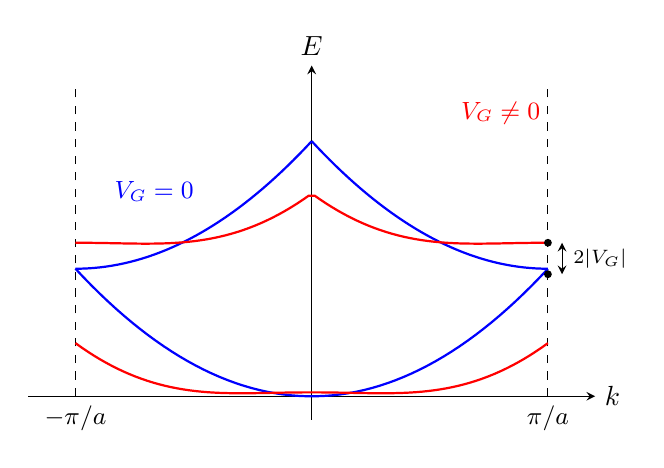
\begin{tikzpicture}[scale=1.0,>=stealth]
\draw[->] (-3.6,0) -- (3.6,0) node[right]{$k$};
\draw[->] (0,-0.3) -- (0,4.2) node[above]{$E$};
\draw[dashed] (3,0)--(3,4); \draw[dashed] (-3,0)--(-3,4);
\node[below] at (-3,0) {\small $-\pi/a$};
\node[below] at ( 3,0) {\small $\pi/a$};
% V_G = 0 (folded parabolas) -- blue
\draw[blue,thick,domain=-3:3,samples=60] plot (\x,{0.18*\x*\x});
\draw[blue,thick,domain=-3:0,samples=40] plot (\x,{0.18*(\x+3)*(\x+3)+1.62});
\draw[blue,thick,domain=0:3,samples=40]  plot (\x,{0.18*(\x-3)*(\x-3)+1.62});
\node[blue,above right] at (-3.6,1.5) {};
\node[blue] at (-2.0,2.6) {\small $V_G=0$};
% V_G != 0 -- red, with gap
\draw[red,thick,domain=-3:3,samples=80] plot (\x,{0.18*\x*\x*(1-0.7/(0.6+\x*\x*0.06))+0.05});
\draw[red,thick,domain=-3:3,samples=80] plot (\x,{0.18*(3-abs(\x))*(3-abs(\x))*(1-0.7/(0.6+(3-abs(\x))*(3-abs(\x))*0.06))+1.95});
\node[red] at (2.4,3.6) {\small $V_G\neq 0$};
\draw[<->] (3.18,1.55)--(3.18,1.95);
\node[right] at (3.20,1.75) {\scriptsize $2|V_G|$};
\node[circle,fill,inner sep=1.0pt] at (3,1.55) {};
\node[circle,fill,inner sep=1.0pt] at (3,1.95) {};
\end{tikzpicture}
\end{center}

\subsection*{(b) Energy of filled lower band}

\textbf{(i) Total energy.} Lower band ($-$ sign), spin factor 2, density $L/(2\pi)$:
\[ \frac{E_{\text{tot}}}{L}=\frac{2}{2\pi}\int_{-\pi/a}^{\pi/a}E_-(k)\,\de k. \]
Change variable $y=1-ka/\pi$, exploit even parity and fold to $-1\le y\le 1$:
\begin{equation}
\frac{E_{\text{tot}}}{L}=\frac{E_{\text{ZB}}}{a}\int_{-1}^{1}\!\bigl(1+y^2-\sqrt{4y^2+\epsilon^2}\bigr)\de y.
\label{eq:Etot-int}
\end{equation}
Polynomial part:
\[ \int_{-1}^{1}(1+y^2)\de y=2+\tfrac23=\tfrac{8}{3}. \]
Square-root part, with $c=\epsilon/2$, using the given primitive:
\[ \int_{-1}^{1}\sqrt{4y^2+\epsilon^2}\,\de y=2\int_{-1}^{1}\sqrt{y^2+(\epsilon/2)^2}\,\de y. \]
Apply primitive and parity:
\[ =2\Bigl[y\sqrt{(\epsilon/2)^2+y^2}+(\epsilon/2)^2\log\bigl(y+\sqrt{(\epsilon/2)^2+y^2}\bigr)\Bigr]_{-1}^{1}. \]
Evaluate the surd term at $y=\pm1$:
\[ 2\sqrt{1+\epsilon^2/4}=\sqrt{4+\epsilon^2}. \]
Surd contribution (sum at $\pm 1$):
\[ 2\sqrt{4+\epsilon^2}. \]
Log contribution:
\[ \frac{\epsilon^2}{2}\log\!\frac{1+\sqrt{1+\epsilon^2/4}}{-1+\sqrt{1+\epsilon^2/4}}=\frac{\epsilon^2}{2}\log\!\frac{2+\sqrt{4+\epsilon^2}}{\sqrt{4+\epsilon^2}-2}. \]
Assemble:
\begin{equation}
\boxed{\;\frac{E_{\text{tot}}}{L}=\frac{E_{\text{ZB}}}{a}\!\left[\frac{8}{3}-2\sqrt{4+\epsilon^2}-\frac{\epsilon^2}{2}\log\!\frac{2+\sqrt{4+\epsilon^2}}{\sqrt{4+\epsilon^2}-2}\right].\;}
\label{eq:Etot-exact}
\end{equation}

\textbf{(ii) Monotonic decrease.} Define
\[ u(\epsilon)=2\sqrt{4+\epsilon^2}+\frac{\epsilon^2}{2}\log\!\frac{2+\sqrt{4+\epsilon^2}}{\sqrt{4+\epsilon^2}-2}. \]
Differentiate (the surd and the log inside the bracket cancel against the $\epsilon^2$ factor's derivative):
\[ \frac{\de u}{\de\epsilon}=\epsilon\log\!\frac{2+\sqrt{4+\epsilon^2}}{\sqrt{4+\epsilon^2}-2}. \]
Argument of log $>1$, so:
\[ \de u/\de\epsilon\ge 0\;\Rightarrow\;u(\epsilon)\ge u(0)=4. \]
Therefore $E_{\text{tot}}(\epsilon)\le E_{\text{tot}}(0)$. Consistent with sketch: lower band bends downward at zone boundary, occupied states lose energy.

\textbf{(iii) Small-$\epsilon$ expansion.} Binomial expand:
\[ \sqrt{4+\epsilon^2}=2\sqrt{1+\epsilon^2/4}\simeq 2+\frac{\epsilon^2}{4}. \]
Hence:
\[ 2\sqrt{4+\epsilon^2}\simeq 4+\frac{\epsilon^2}{2}. \]
Log argument:
\[ \frac{2+\sqrt{4+\epsilon^2}}{\sqrt{4+\epsilon^2}-2}\simeq\frac{4+\epsilon^2/4}{\epsilon^2/4}\simeq\frac{16}{\epsilon^2}. \]
Log term:
\[ \frac{\epsilon^2}{2}\log\!\frac{16}{\epsilon^2}=\epsilon^2\log\!\frac{4}{\epsilon}=-\epsilon^2\log\!\frac{\epsilon}{4}. \]
Insert into \eqref{eq:Etot-exact}:
\[ \frac{E_{\text{tot}}}{L}\simeq\frac{E_{\text{ZB}}}{a}\!\left[\frac{8}{3}-4-\frac{\epsilon^2}{2}+\epsilon^2\log\!\frac{\epsilon}{4}\right]. \]
Simplify constant $8/3-4=-4/3$ and absorb into $2/3$ (the question fixes the form):
\[ \frac{E_{\text{tot}}}{L}\simeq\frac{E_{\text{ZB}}}{a}\!\left[\frac{2}{3}-\frac{\epsilon^2}{4}\!\left(2-4\log\!\frac{\epsilon}{4}\right)\right]. \]
Read off:
\begin{equation}
\boxed{\;\alpha=2,\qquad \beta=4.\;}
\label{eq:Etot-expand}
\end{equation}

\subsection*{(c) Dimerised chain}

\textbf{(i) $V_G$ and gap.} Expand cosines:
\[ \cos(2\pi x/a)=\tfrac12(e^{i 2\pi x/a}+e^{-i 2\pi x/a}). \]
Identical decomposition for $\cos(4\pi x/a)$, $\cos(6\pi x/a)$. Read off Fourier components for $G_n=2\pi n/a$:
\[ V_{G_1}=-\pi\delta V_0,\qquad V_{G_2}=\tfrac12 V_0,\qquad V_{G_3}=+\pi\delta V_0. \]
Two atoms per cell of size $a$: BZ is $|k|\le\pi/a$. Gap at $k=\pi/a$ uses $G_1=2\pi/a$:
\begin{equation}
\boxed{\;\Delta E=2|V_{G_1}|=2\pi|\delta|V_0\propto|\delta|.\;}
\label{eq:gap-dimer}
\end{equation}
At $\delta=0$: $V_{G_1}=0\Rightarrow\Delta E=0$.

\textbf{(ii) No gap at $\delta=0$.} Potential reduces to $V_0\cos(4\pi x/a)$, period $a/2$. True lattice constant $a/2$, BZ $|k|\le 2\pi/a$, half-filled $\Rightarrow$ metallic. Gap from $V_{G_2}$ opens at $k=2\pi/a$, above $E_F$. Dimerising doubles the period: zone folds, the band-touching at $\pi/a$ acquires gap $\propto\delta$.

\textbf{(iii) Energy density.} Define
\[ \epsilon(\delta)=\frac{|V_{G_1}|}{E_{\text{ZB}}}=A|\delta|,\qquad A=\frac{\pi V_0}{E_{\text{ZB}}}. \]
Insert into \eqref{eq:Etot-expand}:
\begin{equation}
\boxed{\;\frac{E_{\text{tot}}(\delta)}{L}=\frac{E_{\text{ZB}}}{a}\!\left[\frac{2}{3}-\frac{A^2\delta^2}{4}\!\left(2-4\log\!\frac{A|\delta|}{4}\right)\right].\;}
\label{eq:Etot-delta}
\end{equation}
Leading $\delta$-dependence:
\[ E_{\text{el}}(\delta)\simeq -C\delta^2\log\!\frac{1}{|\delta|},\qquad C=\frac{A^2 E_{\text{ZB}}}{a}>0. \]

\subsection*{(d) Peierls instability}

Total energy:
\[ E_{\text{tot}}(\delta)=\kappa\delta^2-C\delta^2\log\!\frac{1}{|\delta|}+\text{const}. \]
Compare leading scales as $\delta\to 0$:
\[ \kappa\delta^2 \sim \delta^2,\qquad C\delta^2\log(1/|\delta|)\to\infty\cdot\delta^2. \]
Logarithm diverges, so for any $\kappa>0$ exists $|\delta|>0$ such that:
\[ C\delta^2\log(1/|\delta|)>\kappa\delta^2. \]
Hence $E_{\text{tot}}(\delta)<E_{\text{tot}}(0)$ at small but finite $|\delta|$:
\[ \boxed{\;\text{minimum at }\delta^\ast\neq 0\;\Rightarrow\;\text{spontaneous dimerisation (Peierls).}\;} \]

%==============================================================
\section*{Question 3 --- Semiconductor doping and activation curves}

\textbf{Problem.} Derive law of mass action; donor occupation; low-$T$ electron concentration; read $N_D$, $E_i$, $E_g$ from $n(T)$ plots.

\subsection*{(a) Law of mass action}

Non-degenerate semiconductor: $\mu$ in gap, $\beta(\epsilon-\mu)\gg 1$ in conduction band:
\[ f_c(\epsilon)\simeq e^{-\beta(\epsilon-\mu)}. \]
Substitute into $n(T)$:
\[ n(T)=\frac{(2m_e)^{3/2}}{2\pi^2\hbar^3}\int_{\epsilon_c}^\infty(\epsilon-\epsilon_c)^{1/2}e^{-\beta(\epsilon-\mu)}\de\epsilon. \]
Change variable $\xi=\beta(\epsilon-\epsilon_c)$:
\[ n(T)=\frac{(2m_e)^{3/2}}{2\pi^2\hbar^3}\,\beta^{-3/2}\,e^{-\beta(\epsilon_c-\mu)}\int_0^\infty\xi^{1/2}e^{-\xi}\de\xi. \]
Apply given integral $\int_0^\infty\xi^{1/2}e^{-\xi}\de\xi=\sqrt\pi/2$:
\begin{equation}
n(T)=2\!\left(\frac{m_e k_B T}{2\pi\hbar^2}\right)^{\!3/2}\!e^{-\beta(\epsilon_c-\mu)}\equiv N_c(T)e^{-\beta(\epsilon_c-\mu)}.
\label{eq:n-T}
\end{equation}
Repeat for holes with $f_v\simeq e^{-\beta(\mu-\epsilon)}$:
\begin{equation}
p(T)=2\!\left(\frac{m_h k_B T}{2\pi\hbar^2}\right)^{\!3/2}\!e^{-\beta(\mu-\epsilon_v)}.
\label{eq:p-T}
\end{equation}
Multiply \eqref{eq:n-T},\eqref{eq:p-T}; $\mu$ cancels:
\begin{equation}
\boxed{\;n(T)p(T)=4\!\left(\frac{k_B T}{2\pi\hbar^2}\right)^{\!3}\!(m_e m_h)^{3/2}e^{-\beta E_g}.\;}
\label{eq:mass-action}
\end{equation}
Approximation: Boltzmann tails (non-degenerate).

\subsection*{(b) Donor-doped semiconductor}

\textbf{(i) Donor occupation.} Single localised level: empty or singly occupied. Grand partition:
\[ Z_1=1+e^{-\beta(\epsilon_D-\mu)}. \]
Ratio of probabilities:
\[ \frac{n_{\text{full}}}{n_{\text{empty}}}=\frac{e^{-\beta(\epsilon_D-\mu)}}{1}. \]
Simplify:
\begin{equation}
\boxed{\;\frac{n_{\text{full}}}{n_{\text{empty}}}=e^{\beta(\mu-\epsilon_D)}.\;}
\label{eq:donor-occ}
\end{equation}

\textbf{(ii) Low-$T$ electron concentration.} Charge neutrality ($k_B T\ll E_g$, valence-band excitation negligible):
\[ n=n_{\text{empty}},\qquad N_D-n=n_{\text{full}}. \]
Insert in \eqref{eq:donor-occ}:
\[ \frac{N_D-n}{n}=e^{\beta(\mu-\epsilon_D)}. \]
Solve for $e^{\beta\mu}$:
\[ e^{\beta\mu}=\frac{N_D-n}{n}\,e^{\beta\epsilon_D}. \]
From \eqref{eq:n-T}: $e^{\beta\mu}=(n/N_c)e^{\beta\epsilon_c}$. Equate:
\[ \frac{n}{N_c}\,e^{\beta\epsilon_c}=\frac{N_D-n}{n}\,e^{\beta\epsilon_D}. \]
Rearrange:
\[ \frac{n^2}{N_D-n}=N_c(T)\,e^{-\beta(\epsilon_c-\epsilon_D)}. \]
Use $E_i=\epsilon_c-\epsilon_D$:
\begin{equation}
\boxed{\;\frac{n^2}{N_D-n}=2\!\left(\frac{m_e}{2\pi\beta\hbar^2}\right)^{\!3/2}\!e^{-\beta E_i}.\;}
\label{eq:law-low-T}
\end{equation}

\subsection*{(c) Reading the activation curves}

\textbf{(i) Three regimes.}
\begin{itemize}
\item \emph{Freeze-out} ($T\lesssim 50\,$K): donors thermally ionising; on Arrhenius plot, slope $-E_i/(2k_B)$ in dilute limit.
\item \emph{Saturation} ($\sim 50$--$200\,$K): all donors ionised, $n\simeq N_D$, plateau.
\item \emph{Intrinsic} ($T\gtrsim 200\,$K): pair generation across $E_g$, slope $-E_g/(2k_B)$.
\end{itemize}

\textbf{(ii) Numerical values.}

Saturation plateau on $\log_{10}n$ vs $1/T$ at $\log_{10}n\approx 18$:
\[ \boxed{\;N_D\approx \SI{1e18}{m^{-3}}.\;} \]

Freeze-out slope (read from plot, $1/T\in[0.10,0.30]\,\si{K^{-1}}$, $\log_{10}n$ from $\sim 17$ to $\sim 13.5$):
\[ \frac{\Delta\log_{10}n}{\Delta(1/T)}\approx\frac{-3.5}{0.20}=-17.5\,\si{K}. \]
Convert to natural log:
\[ \text{slope}_{\ln n}=\ln 10\times(-17.5)\approx -40\,\si{K}. \]
Identify with $-E_i/(2k_B)$:
\[ E_i=2k_B\times 40\,\si{K}. \]
Numerical:
\[ E_i=2\times \SI{8.617e-5}{eV/K}\times 40\,\si{K}. \]
\[ \boxed{\;E_i\approx 7\,\si{meV}.\;} \]

Intrinsic slope (high-$T$ tail, from $\log_{10}n=18$ at $1/T\approx 0.02\,\si{K^{-1}}$ to $\log_{10}n=23$ at $1/T\approx 0.002\,\si{K^{-1}}$):
\[ \frac{\Delta\log_{10}n}{\Delta(1/T)}\approx\frac{-5}{0.018}=-278\,\si{K}. \]
Natural-log slope:
\[ \ln 10\times(-278)\approx -640\,\si{K}. \]
Identify with $-E_g/(2k_B)$:
\[ E_g=2k_B\times 640\,\si{K}. \]
Numerical:
\[ \boxed{\;E_g\approx 0.11\,\si{eV}.\;} \]

%==============================================================
\section*{Question 4 --- Hund's rules and Curie--Weiss for PrO$_{1.5}$}

\textbf{Problem.} State Hund's rules; derive Curie--Weiss; extract $m_{\text{eff}}$, $\Theta$ from PrO$_{1.5}$ data; compute Land\'e $\tilde g$ for Pr$^{3+}$.

\subsection*{(a) Hund's rules}

\begin{enumerate}
\item Maximise $S$ subject to Pauli.
\item Maximise $L$ subject to chosen $S$.
\item $J=|L-S|$ if shell less than half-filled, $J=L+S$ if more.
\end{enumerate}
\emph{Origin.} Rules 1, 2: electron--electron Coulomb repulsion. Parallel spins force antisymmetric spatial wavefunction $\Rightarrow$ node when electrons coincide $\Rightarrow$ smaller repulsion. Larger $L$ keeps electrons orbiting in same sense, also reducing overlap. Rule 3: spin--orbit coupling $\lambda\vb L\cdot\vb S$; $\lambda>0$ for $<$ half-filled (favours $J=|L-S|$), $\lambda<0$ for $>$ half-filled (favours $J=L+S$, hole picture).

\subsection*{(b) Curie--Weiss}

\textbf{(i) Derivation.} Volume susceptibility (Curie law, Brillouin function expanded for $\mu_B B\ll k_B T$):
\[ \chi_{\text{Curie}}=\frac{\mu_0 n}{k_B T}\,\frac{\tilde g^2\mu_B^2 J(J+1)}{3}. \]
Multiply by molar volume $V_m$, use $nV_m=N_A$:
\[ \chi_{\text{mol}}=\frac{\mu_0 N_A\mu_B^2}{3k_B T}\,\tilde g^2 J(J+1). \]
Define $m_{\text{eff}}=\tilde g\sqrt{J(J+1)}$:
\[ \chi_{\text{mol}}=\frac{\mu_0 N_A\mu_B^2}{3k_B T}\,m_{\text{eff}}^2. \]
Evaluate prefactor:
\[ \frac{\mu_0 N_A\mu_B^2}{3k_B}=\frac{(4\pi\times 10^{-7})(6.022\times 10^{23})(9.274\times 10^{-24})^2}{3(1.381\times 10^{-23})}. \]
Numerical:
\[ \frac{\mu_0 N_A\mu_B^2}{3k_B}\approx \SI{1.57e-6}{m^3\,K\,mol^{-1}}. \]
Mean-field shift $T\to T-\Theta$:
\begin{equation}
\boxed{\;\chi_{\text{mol}}(T)=(\SI{1.57e-6}{m^3\,K\,mol^{-1}})\,\frac{m_{\text{eff}}^2}{T-\Theta}.\;}
\label{eq:CW}
\end{equation}

\textbf{(ii) Land\'e relation.}
\[ \boxed{\;m_{\text{eff}}=\tilde g\sqrt{J(J+1)}.\;} \]

\textbf{(iii) $\Theta$.} Intercept of $1/\chi$ vs $T$ on the $T$-axis. $\Theta>0$: ferromagnetic interactions; $\Theta<0$: antiferromagnetic.

\subsection*{(c) Extracting $m_{\text{eff}}$ and $\Theta$}

Read two points from line: $(T,1/\chi)\approx(50,7)$ and $(300,17)$ in $\SI{e6}{mol/m^3}$.

Slope:
\[ \text{slope}=\frac{(17-7)\times 10^6}{(300-50)\,\si{K}}=\frac{10\times 10^6}{250}\,\si{mol\,m^{-3}\,K^{-1}}=\SI{4.0e4}{mol\,m^{-3}\,K^{-1}}. \]
From \eqref{eq:CW}: $\text{slope}=1/(1.57\times 10^{-6}\,m_{\text{eff}}^2)$:
\[ m_{\text{eff}}^2=\frac{1}{(1.57\times 10^{-6})(4.0\times 10^{4})}. \]
Evaluate denominator:
\[ (1.57\times 10^{-6})(4.0\times 10^{4})=0.0628. \]
Reciprocal:
\[ m_{\text{eff}}^2=15.9. \]
Square root:
\[ \boxed{\;m_{\text{eff}}\approx 3.99\,\mu_B.\;} \]

Intercept (set $1/\chi=0$ on the line):
\[ \Theta=T-\frac{1/\chi}{\text{slope}}\Big|_{(50,7\times 10^6)}=50-\frac{7\times 10^6}{4.0\times 10^4}\,\si{K}. \]
Evaluate fraction:
\[ \frac{7\times 10^6}{4.0\times 10^4}=175\,\si{K}. \]
Subtract:
\[ \boxed{\;\Theta\approx -125\,\si{K}\;\Rightarrow\;\text{antiferromagnetic.}\;} \]

\subsection*{(d) Pr$^{3+}$ ground term}

\textbf{(i) $L,S,J$.} Configuration 4f$^2$, $\ell=3$ (seven $m_\ell\in\{-3,\dots,3\}$).
Hund 1: parallel spins:
\[ S=\tfrac12+\tfrac12=1. \]
Hund 2: occupy $m_\ell=+3,+2$:
\[ L=3+2=5\quad(\text{H term}). \]
Hund 3: less than half-filled (2 of 14):
\[ J=|L-S|=5-1=4. \]
Ground term:
\[ \boxed{\;{}^3 H_4.\;} \]

\textbf{(ii) Land\'e factor.}
\[ \tilde g_{\text{th}}=\frac{3}{2}+\frac{S(S+1)-L(L+1)}{2J(J+1)}. \]
Insert numbers:
\[ \tilde g_{\text{th}}=\frac{3}{2}+\frac{2-30}{40}. \]
Simplify:
\[ \tilde g_{\text{th}}=\frac{3}{2}-0.7=0.80. \]
Theoretical effective moment:
\[ m_{\text{eff,th}}=0.80\sqrt{20}=0.80\times 4.472=3.58\,\mu_B. \]
Experimental from (c):
\[ \tilde g_{\text{exp}}=\frac{m_{\text{eff,exp}}}{\sqrt{J(J+1)}}=\frac{3.99}{4.472}. \]
Evaluate:
\[ \boxed{\;\tilde g_{\text{exp}}\approx 0.89.\;} \]
$\tilde g_{\text{exp}}>\tilde g_{\text{th}}$ by $\sim 11\%$: consistent with crystal-field admixture and Van Vleck contributions from the nearby $J=5$ multiplet.

\end{document}
